\chapter{Исследовательская часть}

\section{Оборудование}

Характеритстики ноутбука:
\begin{itemize}
	\item Процессор intel-core i5-12500H
	\item ОЗУ 16 Гб DDR4
	\item ОС Windows 11
\end{itemize}

Цель исследования: разобраться, как происходит сравнение тектов на похожесть. Изучить методы сравнения текстов.

Исследование происходило при подключенном кабеле питания, при выключенных сторонних приложениях.

\section{Графики}

\begin{figure}[H]
    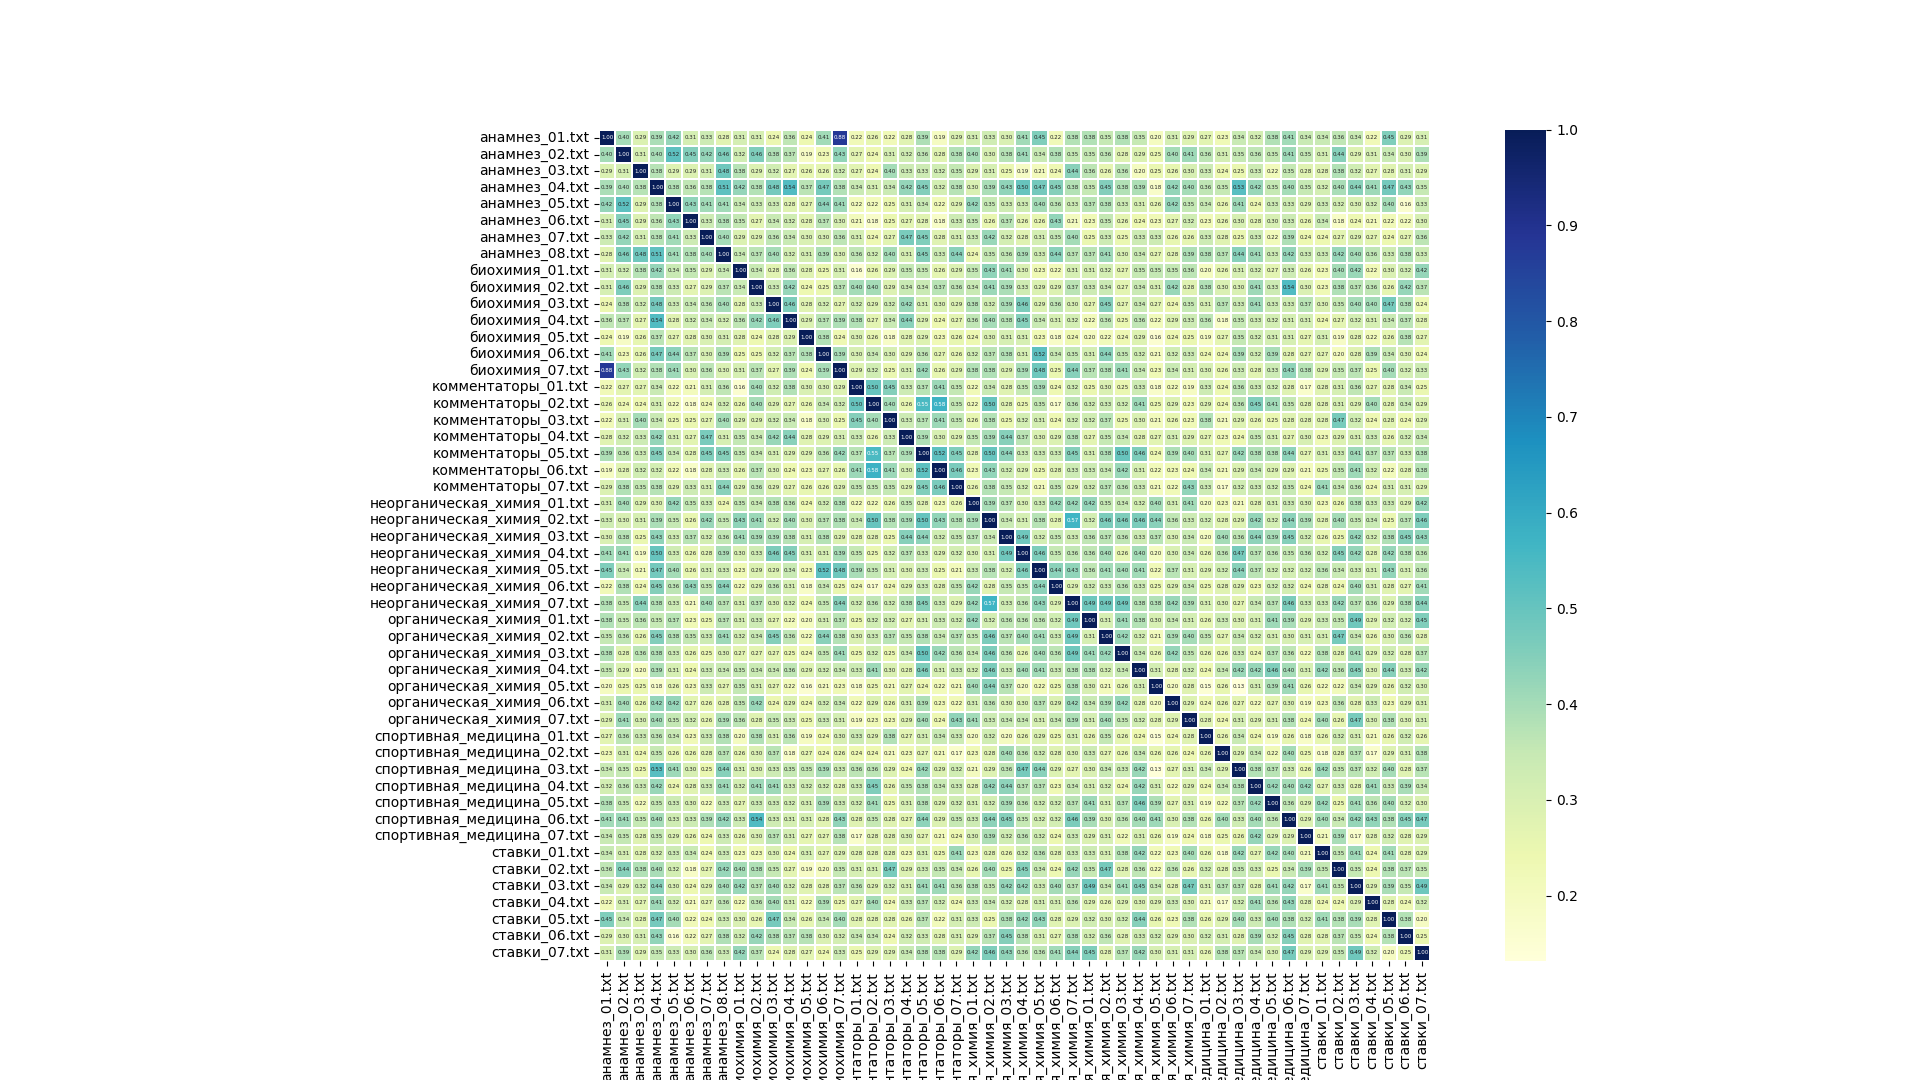
\includegraphics[width=1.1\textwidth]{C:/MGTU/baseAI/lr7/results/HeatmapJac.png}
    \caption{Карта сравнения документов методом Жаккара}
    \label{fig:one}
\end{figure}

\begin{figure}[H]
    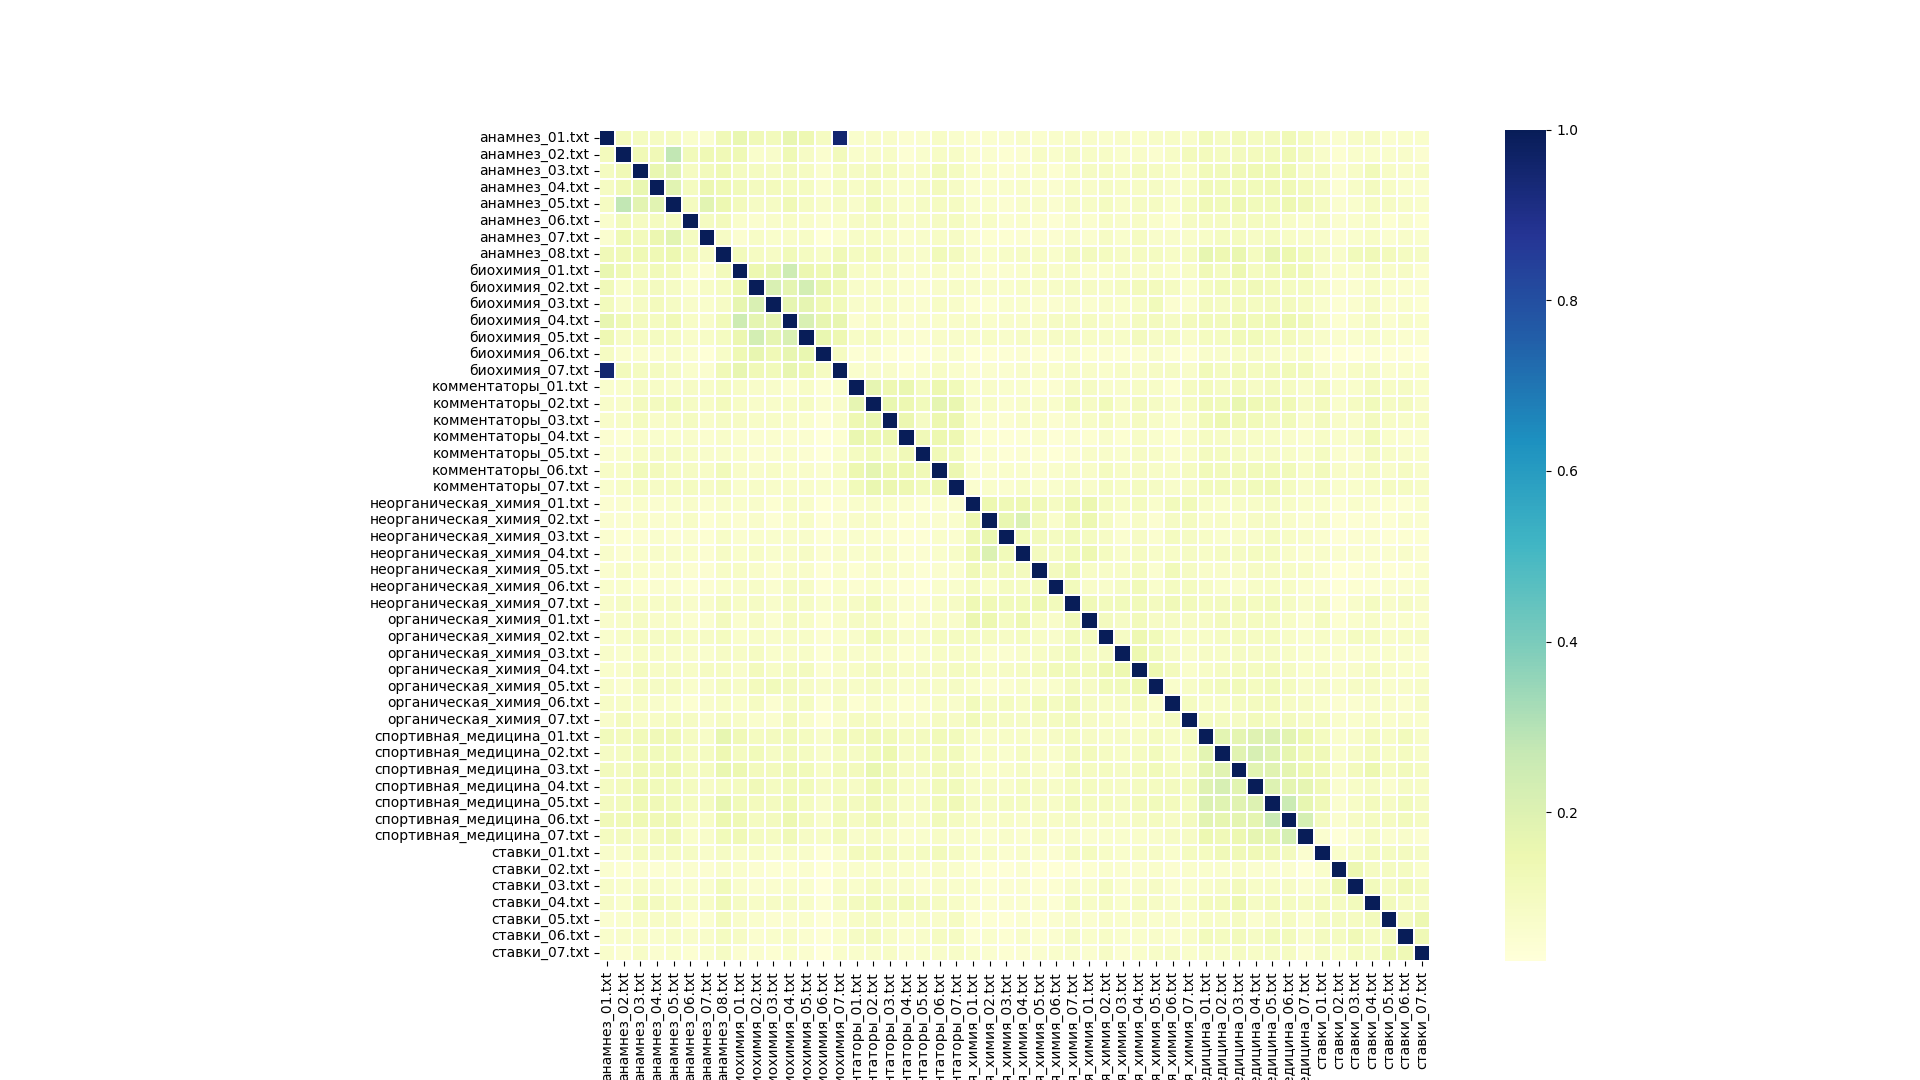
\includegraphics[width=1.1\textwidth]{C:/MGTU/baseAI/lr7/results/HeatmapJacNorm.png}
    \caption{Карта сравнения документов методом Жаккара, нормализированный}
    \label{fig:one}
\end{figure}

\begin{figure}[H]
    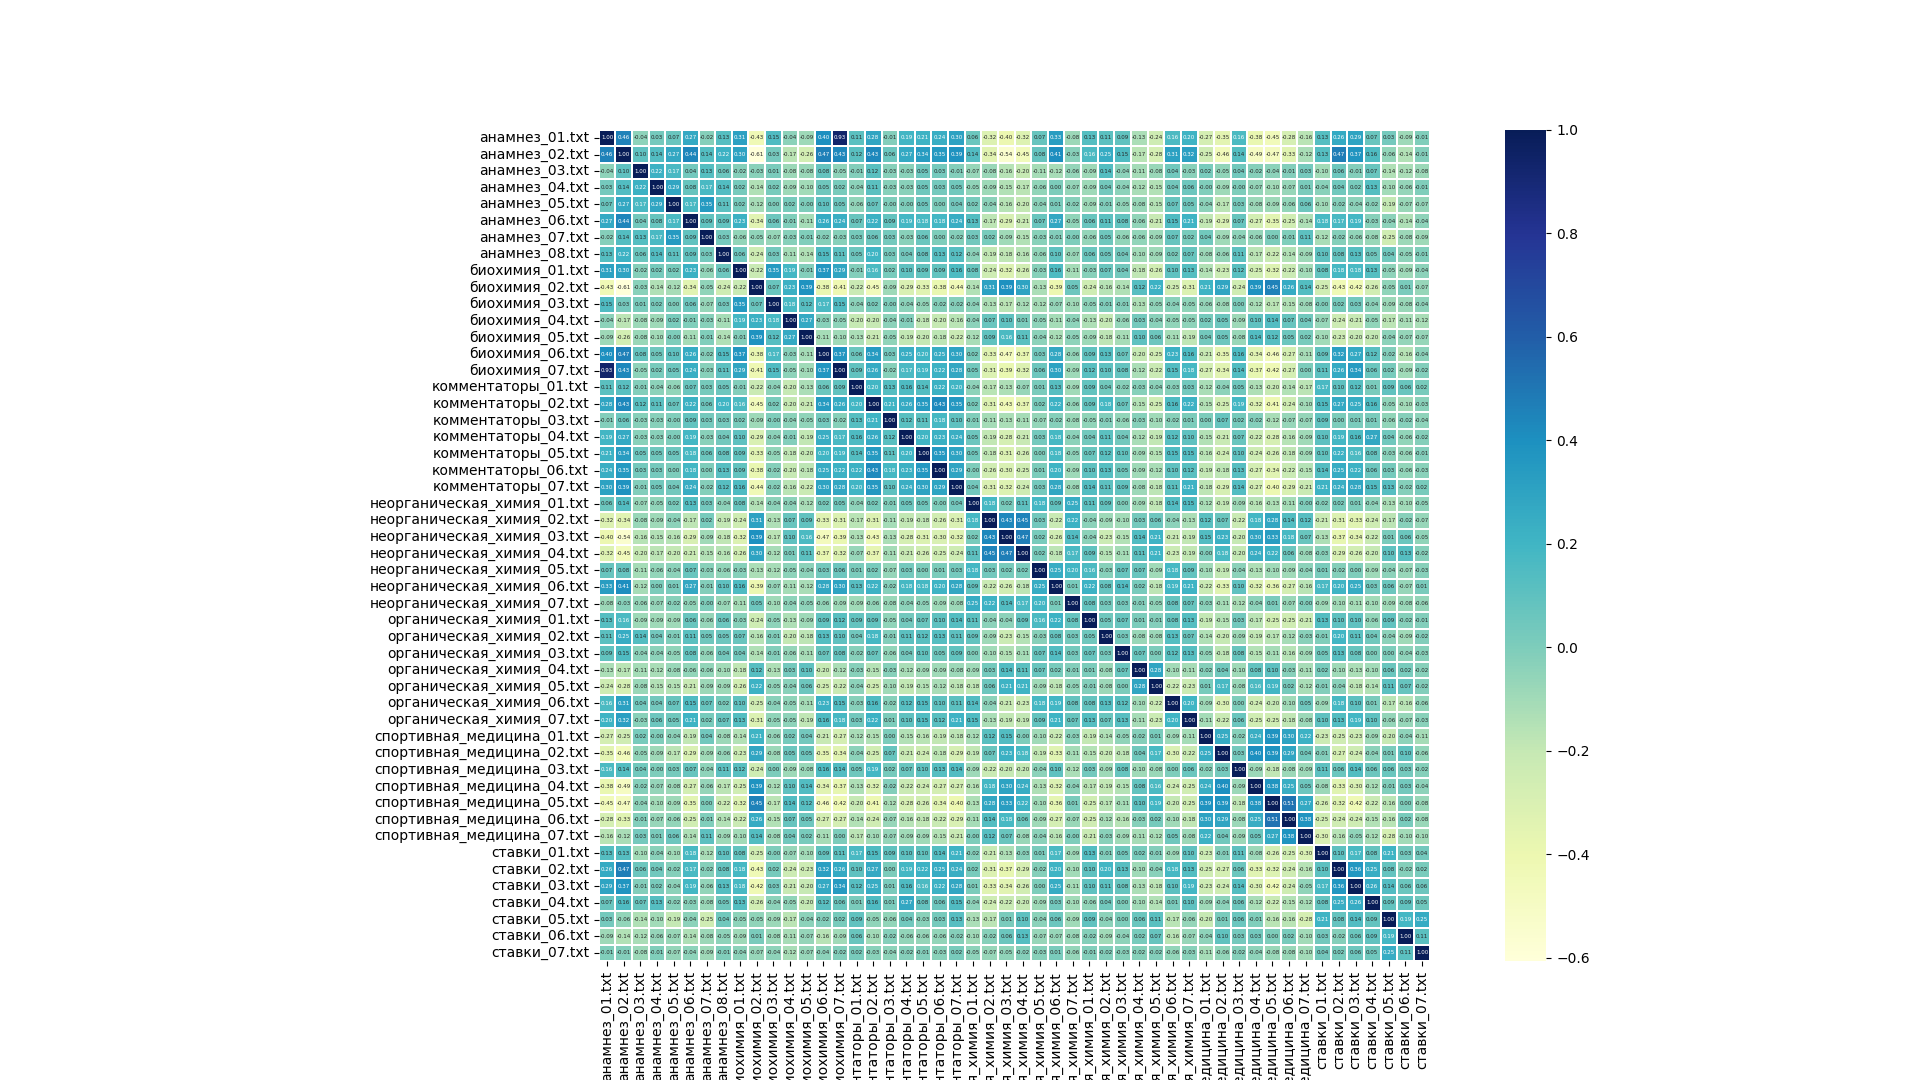
\includegraphics[width=1.1\textwidth]{C:/MGTU/baseAI/lr7/results/HeatmapCos.png}
    \caption{Карта сравнения документов косинусной мерой близости}
    \label{fig:one}
\end{figure}

\begin{figure}[H]
    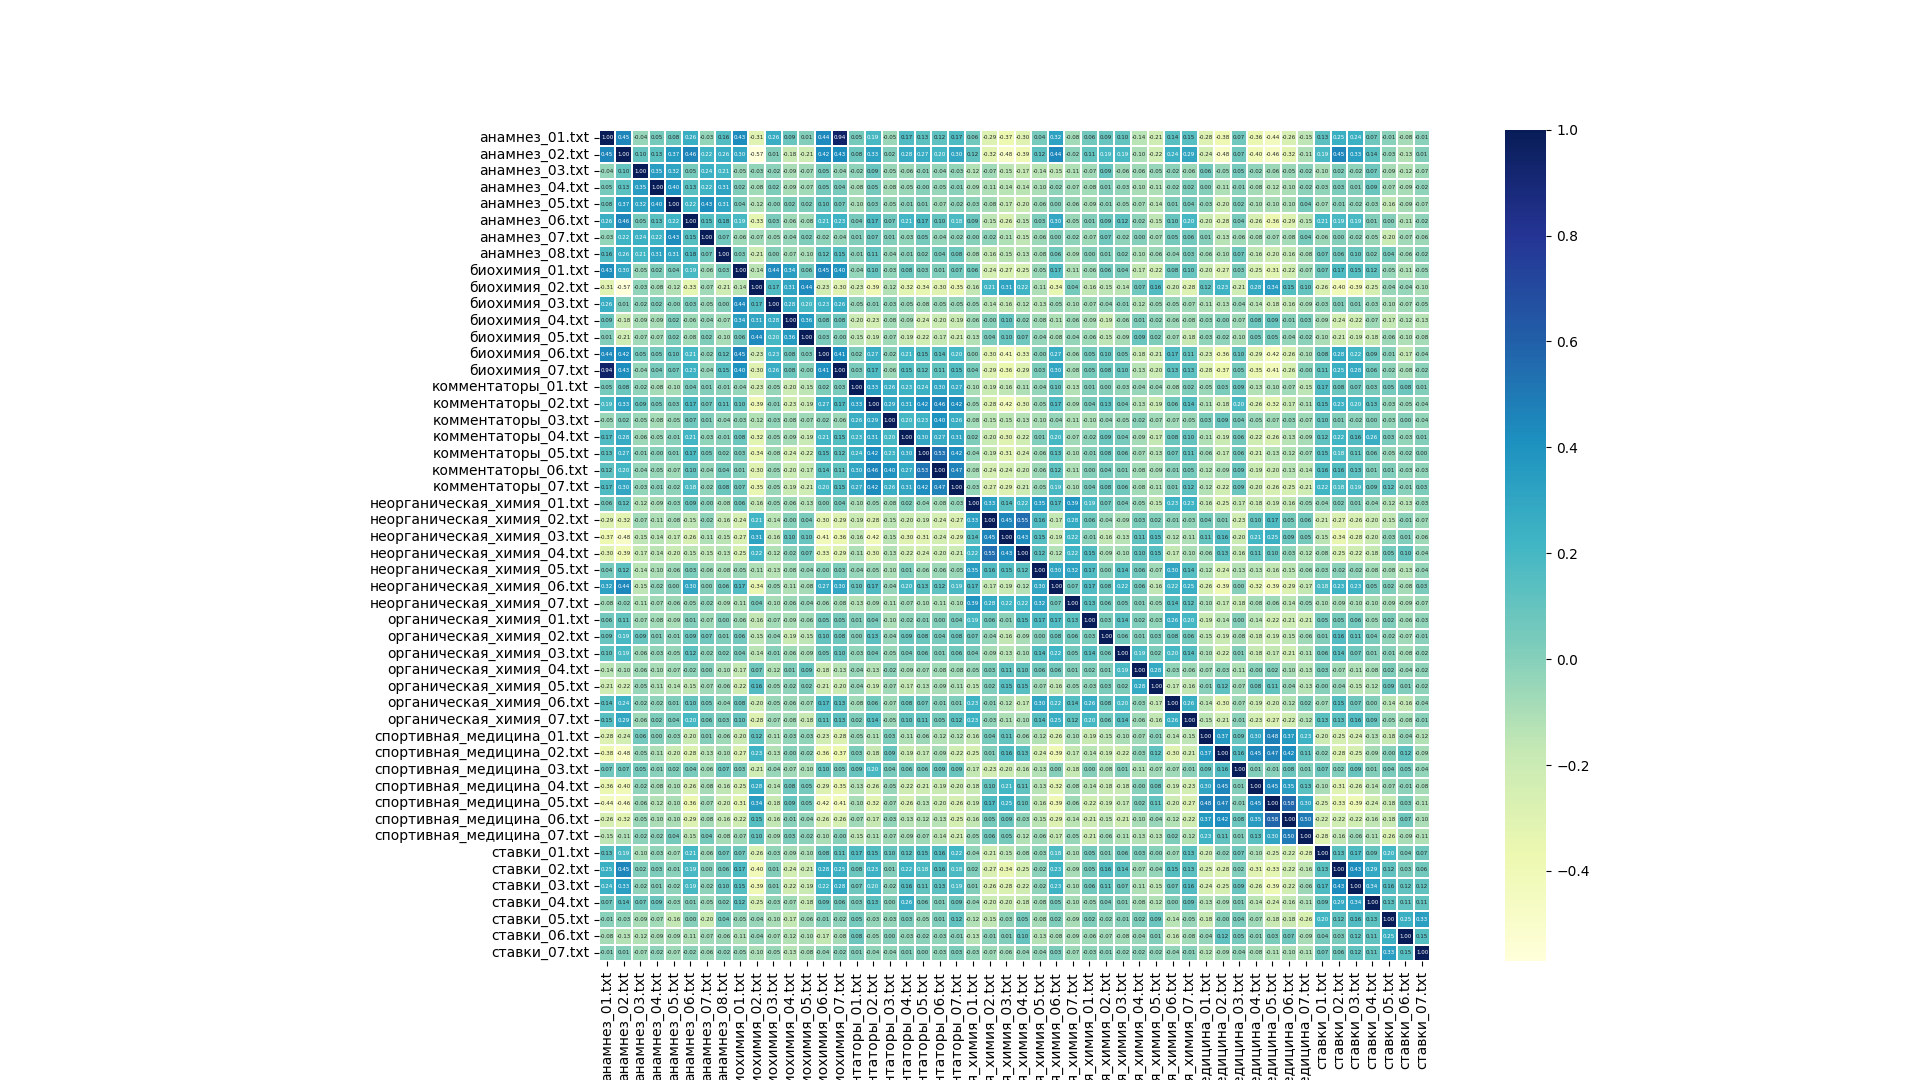
\includegraphics[width=1.1\textwidth]{C:/MGTU/baseAI/lr7/results/HeatmapCosNorm.png}
    \caption{Карта сравнения документов  косинусной мерой близости, нормализированный}
    \label{fig:one}
\end{figure}

\section{Вывод}

В результате исследования наилучшим образом показал себя косинусный метод сравнения. На графике четко видна степень различия файлов.
Метод Жаккара практически не показывает разницу между текстами.

Нормализированные вектора абсолютно не меняют рисунок графика, только усиливают корреляцию файлов.

\clearpage
